\documentclass[a4paper]{article}
\usepackage[utf8]{vietnam, inputenc}
\usepackage[english]{babel}
\usepackage{amsmath, amssymb, anyfontsize, array, bookmark, caption, color, comment, enumerate, enumitem, fancyhdr, float, graphicx, hyperref, lastpage, listings, mathtools, pgfplots, pifont, systeme, tikz}
\usepackage[framemethod=tikz]{mdframed}
\usetikzlibrary{calc, backgrounds}
\newcommand\HRule{\rule{12cm}{1pt}}
\pagestyle{fancy}
\fancyhead{} % clear all header fields
\fancyhead[L]{
	\color{blue}
	\begin{tabular}{rl}
		\begin{picture}(25,15)(0,0)
		\put(0,-8){
\includegraphics[width=8mm, height=8mm]{BK.png}}
		\end{picture}
		\begin{tabular}{l}
			\textbf{\bf \ttfamily Ho Chi Minh University of Technology}\\
			\textbf{\bf \ttfamily Faculty of Computer Science \& Engineering}
		\end{tabular} 	
	\end{tabular}
}
\fancyhead[R]{
	\begin{tabular}{l}
		\tiny \bf \\
		\tiny \bf 
	\end{tabular}
}
\fancyfoot{} % clear all footer fields
\fancyfoot[L]{\scriptsize \ttfamily Calculus 2 Assignment}
\fancyfoot[R]{\scriptsize \ttfamily Page {\thepage}/\pageref{LastPage}}
\renewcommand{\headrulewidth}{0.3pt}
\renewcommand{\footrulewidth}{0.3pt}

\definecolor{dkgreen}{rgb}{0,0.6,0}
\definecolor{gray}{rgb}{0.5,0.5,0.5}
\definecolor{mauve}{rgb}{0.58,0,0.82}

\lstset{frame=tb,
	language=Matlab,
	aboveskip=3mm,
	belowskip=3mm,
	showstringspaces=false,
	columns=flexible,
	basicstyle={\small\ttfamily},
	numbers=none,
	numberstyle=\tiny\color{gray},
	keywordstyle=\color{blue},
	commentstyle=\color{dkgreen},
	stringstyle=\color{mauve},
	breaklines=true,
	breakatwhitespace=true,
	tabsize=3,
	numbers=left,
	stepnumber=1,
	numbersep=1pt,    
	firstnumber=1,
	numberfirstline=true
}
\begin{document}
\begin{titlepage}
	
\begin{tikzpicture}[remember picture, overlay]
		\draw[line width = 2pt] ($(current page.north west) + (1in,-1in)$) rectangle ($(current page.south east) + (-1in,1in)$);
	\end{tikzpicture}
	
	\begin{center}

		% Upper part of the page
		\textbf{\fontsize{12pt}{1pt}\selectfont HO CHI MINH CITY UNIVERSITY OF TECHNOLOGY}\\[0.5cm]
		{\fontsize{13pt}{1pt}\selectfont Faculty of Computer Science \& Engineering}\\[0.5cm]
		\begin{figure}[h]
			\centering
			
\includegraphics[width=1.7in,height=1.7in]{BK.png}
		\end{figure}
		
		% Title
		\HRule \\[0.5cm]
		{ \textbf{\fontsize{25pt}{1pt}\selectfont Calculus 2 Assignment}}\\[0.4cm]
		
		\HRule \\[0.8cm]
		\begin{minipage}{0.545\textwidth}
			\begin{flushleft} 
				\textbf{Authors:}\\
				\begin{tabular}{l l}
					Nguyễn Hoàng  & 1952255 \\
					Tạ Minh Huy   & 1952268 \\
					Ho Trí Kháng  & 1952069 \\
					Nguyễn Khương & 1952310 \\
					Lê Minh Đăng  & 1952041 \\
					Đỗ Đăng Khoa  & 1952295
				\end{tabular}
			\end{flushleft}
		\end{minipage}
		\begin{minipage}{0.4\textwidth}
			\begin{flushright} 
				\textbf{Class:}\\
				MT1006\\
				\textbf{Lecturer:}\\
				Phan Thị Khánh Vân\\
				
			\end{flushright}
		\end{minipage}
		
		\vfill
		
		% Bottom of the page
		\vspace{2cm}
		{\large} %{\large \today}
	\end{center}
\end{titlepage}

\thispagestyle{empty}
\newpage
\tableofcontents
\newpage

\pdfbookmark[0]{Partial Derivatives}{PartDeriv}
\section{Partial Derivatives}
Partial Derivative or PDEs is one of the most common concept in Mathematics. In real life, it is applied widely in several fields, from Physics, Mathematics, Economics or Engineering, etc. \\
In this paper, let's consider one of the most popular applications of Partial Derivatives in Economics, Marginal Analysis
\pdfbookmark[1]{Marginal Analysis}{marginal}
\subsection{Marginal Analysis}

\textit{Marginal analysis is an examination of the additional benefits of an activity compared to the additional costs incurred by that same activity.} \\ \\
Let's first make it simpler by the following example. \\
\emph{The total profit that a company makes is represented in a function p(x,y), where x, y is numbers of units of sale made on 2 goods x, y respectively. If either x or y increases (or decreases), it will affect the total outcome of that company.} \\ \\
By taking the derivative of $p$ with respect to $x$ $\frac{dp}{dx}$ (treating y as constant), we obtain the relationship on how the change of $x$ affects the profit $p$. That is, how much incremental profit is attained when one more unit of $x$ is sold. In other words, the result we obtain when taking Partial Derivatives of $p$ with respect to $x$ is called the marginal effect that $x$ has on $p$. \\ \\
In other words, Marginal Analysis is evaluating how the increase and decrease of inputs will affect the total output.\\ \\
In Marginal Analysis, the concept of marginal utility is the added satisfaction that a consumer has when consuming additional units of goods or services. \\ \\
Assume a utility function follows the formula
\begin{equation*}
	u(x,y) = x^{0.4}\cdot y^{0.6}
\end{equation*}
where x,y are the unit of two goods consumed by consumers.\\ \\
The marginal utilities of x and y, $MU_X$ and $MU_Y$ can be found by taking the first order PDEs of u with respect to $x$ and $y$, respectively.\\
To obtain $u'_x$, fix $y$ (y is considered as constant), and differentiate function with respect to x: 
\begin{align*}
	MU_x & = \frac{du}{dx} = 0.4x^{-0.6}y^{0.6} 
\end{align*}
Similarly for y:
\begin{align*}
	MU_y & = \frac{du}{dy} = 0.6x^{0.4}y^{-0.4}
\end{align*}
We can use MATLAB software to make things easier:
\begin{figure}[H]
	\centering
	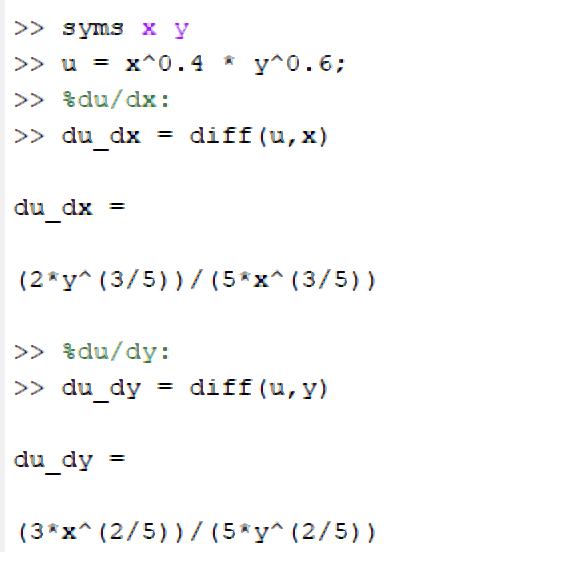
\includegraphics[width=0.6\textwidth]{PDE1.png}
\end{figure}

Economists and analysts use these calculations to make business decisions:
\begin{enumerate}[label=$\bullet$]
	\item Both $MU_x$ and $MU_y$ are positive, they are positive marginal utilities. When the total utility is low, the consumption of an additional unit of goods will likely to increase the total utility.
	\item However, when the total utility grows, increasing $x$ and $y$ may produce slower rates of increased total utility. Like when you use a service several times, your satisfaction to that service becomes less and less compared to first times you use it.
	\item When it reaches a specific point, the total utility stops growing, the marginal utility becomes zero. Increasing input will not make the total output increase, but remain stable. We can demonstrate this by taking limit of $du/dx$ (or $du/dy$):
	      \begin{equation*}
		      \lim\limits_{x \to +\infty} 0.4x^{-0.6}\cdot y^{0.6} = 0
	      \end{equation*}
	      In fact, the total output starts to decrease, as the satisfaction of consumers gradually reduces, the marginal utility becomes negative. 
	\item Economists will have to avoid negative utilities in most cases, and make proper calculations to maximize the effectiveness of their tasks.
\end{enumerate}
Lets take another example where PDEs can be applied to marginal production: \\
\emph{The total production $P$ of a certain product depends on the amount of labor $L$ used and the amount $K$ of capital investment. Assume that $P$ follows the Cobb-Douglas model, given by the formula:}
\begin{equation*}
	P = 10K^{2/3}L^{1/3}
\end{equation*}
The task is to find the marginal product of capital $MP_K$ and marginal product of labor $MP_L$, obtained by taking the first-order partial derivatives of $P$ with respect to $K$ and $L$, respectively. \\
Using software makes things more straightforward:
\begin{figure}[H]
	\centering
	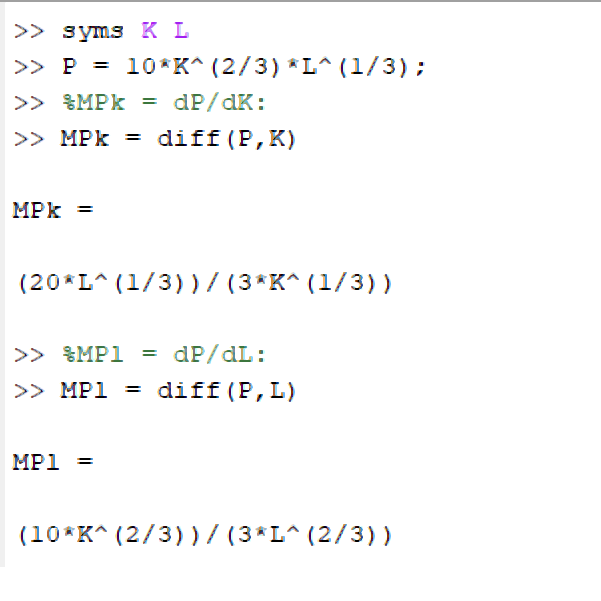
\includegraphics[width = 0.6\textwidth]{PDE2.png}
\end{figure}
\begin{align*}
	MP_K & = \frac{20}{3} \cdot L^{\frac{1}{3}} K^{\frac{-1}{3}} \\
	MP_L & = \frac{10}{3} \cdot K^{\frac{2}{3}} L^{\frac{-2}{3}}
\end{align*}
The analysis of economists is the same as mentioned in previous example about marginal utility: The increase in investment of labor and capital at first will likely to increase the total product. This rate decreases gradually and will reach 0 at a specific point, which produces a zero marginal product. \\
\subsubsection*{Optimization:}
In fact, the task of economists is not just simply calculate marginal product. They are asked to do more complicated tasks. For instance, the work is finding an optimal strategies that maximizes the total production of their company. \\
Fortunately, Mathematics gives them some useful tools to tackle this problem, one of which is Lagrange Multipliers. \\
To deal with this task, there are often some restrictions or economic constraints that can be used to produce optimal solution.\\
Let’s get back to the Cobb Douglas formula mentioned before:
\begin{equation*}
	P = 10K^{2/3}L^{1/3}
\end{equation*}
Suppose a company want to maximize the total product P. They can spent a maximum total budgets of \$24000 for labor and capital investment. Given that the cost of a unit of labor is \$4, and the cost of a unit of capital is \$8.  How many units of labor and capital should they consider? \\
Lets review some key points about Lagrange Multiplier: \\
\begin{itemize}
	\item Suppose that $x_0$,$y_0$ is an extremum of $z = f(x,y)$ subject to the constraint $\Phi(x,y) = k$. We define the Lagrange function:
	      \begin{equation*}
		      L(x,y,\lambda) = f(x,y) - \lambda[\Phi(x,y) - k]
	      \end{equation*}
	\item If we differentiate both sides of Lagrange equation above with respect to $x$, $y$ and $\lambda$, we obtain a system of equations. The solution of that system is the extremum of the function z.
	\item Remember that Lagrange method is applied only when both $z(x,y)$ and $\Phi(x,y)$ have continuous first Partial Derivatives on domain D.
\end{itemize}
Applied to the optimization problem that we are considering above: \\
The constraint equation:
\begin{equation*}
	8K + 4L  = 24000
\end{equation*}*
where $\Phi(x,y) = 8K + 4L$ \\
Both $P$ and $g$ have continuous PDEs (as $K$ and $L$ > 0). We define Lagrange function:
\begin{equation*}
	L(x,y,\lambda) = 10K^{2/3}L^{1/3} - \lambda(8K + 4L -24000)
\end{equation*}
Taking PDEs of $L$ with respect to $x$,$y$ and $\lambda$, we obtain the system of equations:
\[
	\systeme{\frac{20}{3} \cdot L^{\frac{1}{3}} K^{\frac{-1}{3}} = 8\lambda ,\frac{10}{3} \cdot K^{\frac{2}{3}} L^{\frac{-2}{3}}  = 4\lambda , 8K + 4L  = 24000}
\]
It can be seen that equations are determined only when $\lambda$ $\neq$ 0 . Dividing equation 1 to equation 2($L$ and $K$ must be greater than 0) , we obtain a new system:
\[
	\systeme{2\frac{L}{K} = 2, 8K + 4L = 24000}
\]
The solution is K = 2000, L = 2000. Substituting L and K to the first equation: $\lambda = -0.833 $. \\
Substituting L and K to the product function, we obtain $P$ = \$20000. \\
The maximum of product $P$ is \$20000 when L = K = \$2000. \\
We can use MATLAB to implement Lagrange method, finding the maximum product:
\begin{figure}[H]
	\centering
	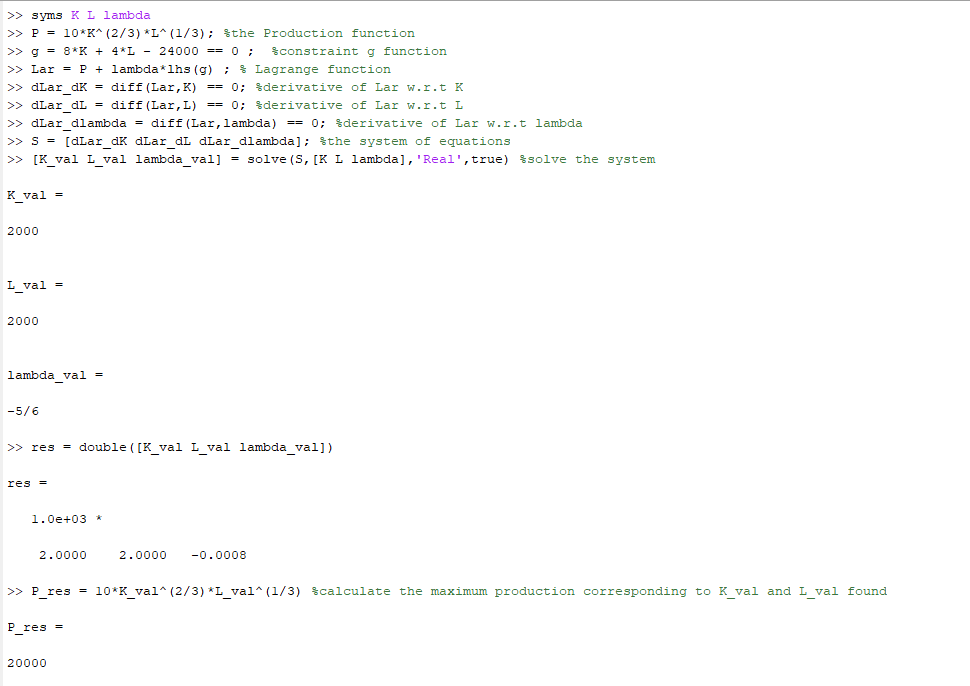
\includegraphics[width=1\textwidth]{PDE3.png}
\end{figure}
The technique of Partial Differentiation makes many economic problem become much more easy. \\
Marginal Analysis helps economists to keep up with the economy , where Partial Derivatives plays a crucial role. \\ Therefore, economists can think of smart strategies that can maximize the total product.
\newpage
\pdfbookmark[0]{Multiple Integrals}{MultInt}
\section{Multiple Integral}
\subsection{Double Integral in rainfall calculation}
\begin{enumerate}[label=\textbf{$\alph*.$}]
	\item Fubini's Theorem\cite{anton2010calculus} in iterated integral to double integral \\
	      Suppose that $f(x,y)$ is a function of two variables that is continuous on a rectangular region $R=\{(x,y)\in \mathbb{R}^2|a\leq x\leq b, c\leq y\leq d\}$. The double integral of $f$ over the region equals to the iterated integral
	      \begin{equation*}
		      \iint f(x,y)\;dx\;dy = \int_a^b \int_c^d f(x,y)\;dy\;dx = \int_c^d \int_a^b f(x,y)\;dx\;dy
	      \end{equation*}
	      
	\item Double Integral \\
	      The double integral of $f$ over the rectangle R is
	      \begin{equation*}
		      \iint f(x,y)\;dA = \lim_{m,n \rightarrow \infty} \sum_{i=1}^{m} \sum_{j=1}^{n} f(x_{ij}^{*}, y_{ij}^{*})\; \Delta A
	      \end{equation*}
	      if this limit exists.
\end{enumerate}
There are many applications of double integral such as: Calculating the surface area, volume of elliptic paraboloid, calculating the probability, center of mass, mass... but there is an application of calculating the storm rainfall using the definition of double integral, which is very useful for meteorologists. It helps them effectively measure the rainfall and reduce the errors as in the average method.

\pdfbookmark[1]{Calculating the Rainfall}{rainfall}
\textit{For example: } Calculate the rainfall from the remnants of Hurricane Karl of the Midwest on September 22-23th, 2010. The area of rainfall measured 300 miles east to west and 250 miles north to south. Estimate the average rainfall over the entire area in those two days.
\begin{figure}[H]
	\centering
	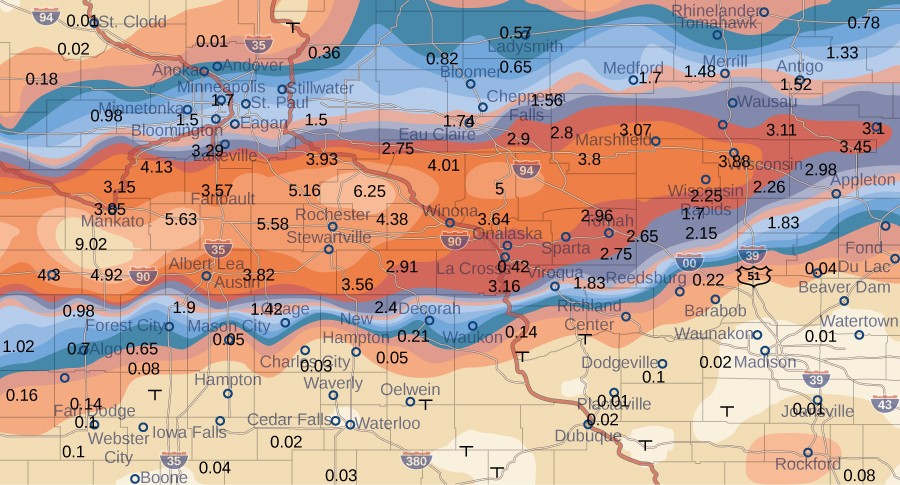
\includegraphics[width=0.8\textwidth]{rain1.png}
\end{figure}
We assume the area of this region is $A$.
\begin{align*}
	A & = 300 \cdot 250 \\
	  & = 75000
\end{align*}
We divide the region into 6 smaller regions
\begin{align*}
	\Delta A & = \frac{1}{6}A \\
	         & = 12500
\end{align*}
Assume that $(x_{ij}^{*}, y_{ij}^{*})$ is the midpoint of each small region, we can estimate the value of each.
\begin{figure}[H]
	\centering
	\includegraphics*[width=0.8\textwidth]{rain2.png}
\end{figure}
Assume $f(x,y)$ denotes the approximate storm rainfall in inch at a point $x$ miles to the east and $y$ miles to the north of the origin. We will estimate the rainfall using two criteria:
\begin{enumerate}[label=$\cdot$]
	\item Points at the same altitude are nearly equal to each other
	\item If point $X$ is near the shore, the value of the point $X$ is the average of value of points on the shoreline and near $X$ and at the same height as $X$ but not on the shoreline.
\end{enumerate}
\begin{enumerate}[label=$\bullet$]
	\item At $(x_{11}, y_{11})$, the rainfall is $0.08$.
	\item At $(x_{12}, y_{12})$, the rainfall is $\frac{0.05+0.14+0.21}{3}=0.13$.
	\item At $(x_{13}, y_{13})$, the rainfall is $\frac{0.01+0.02+0.01}{3}=0.01$.
	\item At $(x_{21}, y_{21})$, the rainfall is $\frac{0.98+1.5+1.7}{3}=1.39$.
	\item At $(x_{22}, y_{22})$, the rainfall is $1.74$.
	\item At $(x_{23}, y_{23})$, the rainfall is $\frac{2.98+3.11}{2}=3.05$.
\end{enumerate}
\begin{align*}
	f_{average} & = \frac{1}{A}\iint f(x,y)\;dx\;dy                                                    \\
	            & \approx \frac{1}{75000} \sum_{1}^{3} \sum_{1}^{2} f(x_{ij}^{*}, y_{ij}^{*}) \Delta A \\
	            & \approx \frac{1}{75000} \begin{multlined}[t]
		\bigl[f(x_{11}, y_{11}) \Delta A + f(x_{12}, y_{12}) \Delta A + f(x_{13}, y_{13}) \Delta A \\
			+ f(x_{21}, y_{21}) \Delta A + f(x_{22}, y_{22}) \Delta A + f(x_{23}, y_{23}) \Delta A\bigr]
	\end{multlined}                               \\
	            & = \frac{1}{75000} \cdot [0.08 + 0.13 + 0.01 + 1.39 + 1.74 + 3.05] \Delta A           \\
	            & = \frac{1}{75000} \cdot [0.08 + 0.13 + 0.01 + 1.39 + 1.74 + 3.05]\; 12500            \\
	            & \approx 1.067\;\text{(inch)}
\end{align*}
We can also use MatLab and the definition of double integral to solve this problem.
\begin{mdframed}[hidealllines=true,backgroundcolor=magenta!10]
	rain.m
	\begin{lstlisting}
		area = 300 * 250;
		a = 1 ./ area;
		smallarea = area ./ 6;
		A = [0.08 0.13 0.01; 1.39 1.74 3.05];
		sum = 0;
		
		for i = 1:1:2
			for j = 1:1:3
				sum = sum + A(i,j);
			end
		end
		
		result = sum * smallarea * a;
		\end{lstlisting}
\end{mdframed}
And the result is $1.0667$.

We can see that this method is easy with the help of double integral. To get the real rainfall using this, we don't need to get the rainfall of each individual location of the area, we just need to know the midpoint of the region or somewhere with highest rainfall of each small region.

\newpage
\pdfbookmark[1]{Probability}{probability}
\subsection{Double Integral in Probability}
\subsubsection*{Introduction of integral in probability:}
\begin{enumerate}
	\item \textbf{Random Variable:} A random variable is a quantity that can take on several different values, depending on chance. For example: \\
	      -The number of football games that the HAGL will win. \\
	      -Tomorrow's high temperature in Ho Chi Minh city. \\
	      The first example is discrete random variables, meaning that you make a list of all the possible outcomes, and then assign a number, called the probability, to each one. The second one continuous random variables, meaning that the possible outcomes form a continuous range.
	\item \textbf{The Probability Density Function:} \\
	      If X is a continuous random variable, then the probability of any one outcome is zero. Instead, we consider the probability of a range of outcomes. The probability density function f(x) gives the probability per unit length. \\
	      Probability density functions can be used to determine the probability that continuous random variable lies between two values a and b, which is computed :
	      \begin{equation*}
		      P ( a \leq X \leq b) = \int_{a}^{b} f(x) dx
	      \end{equation*}
	      And it must satisfies 2 conditions:
	      \begin{itemize}
		      \item $f(x) \geq 0$ $\forall x $
		      \item $\int_{-\infty}^{+\infty} f(x) dx = 1$
	      \end{itemize}
	\item \textbf{Mean value and Variance:} \\
	      If X is a random variable, the expectation or mean value of X is the average value we get when we run the experiment over and over again. Which can be computed : 
	      \begin{equation*}
		      E(X) = \mu =  \int_{-\infty}^{+\infty} xfX(x)dx
	      \end{equation*}
	      Therefore, the Variance - which is the measurement of how wide the distribution is - is calculated as follows:
	      \begin{equation*}
		      Var(X) = E(X^{2}) - \mu ^{2} = \int_{-\infty}^{+\infty} x^{2}fX(x)dx - \mu ^{2}
	      \end{equation*}
	      $\sigma = \sqrt{Var(X)}$ is called the standard deviation of X.
	      
\end{enumerate}
\subsubsection*{Double Integrals in Probability:}
Often, we are interested in two random variables X and Y in a same plane, and want to understand how they are related. For instance: \\
-X might be tomorrow's high temperature, and Y might be tomorrow's barometric pressure. \\
-X might be the concentration of virus in a patient's blood, and Y might be the concentration of an antibody. \\
-X and Y might be the horizontal and vertical coordinates of the spot where a dart hits a board. \\
This is when the application of double integral comes into play, when we have two random variables X and Y, the pair (x,y) takes values in the plane, and we speak of the probability per unit area of (x,y) landing in a certain region. This is called the joint probability density function, and is written f(x,y). \\ \\
The Probability of (X,Y) landing in a region R is:
\begin{equation*}
	P(X,Y \in R ) = \int \int_{R} f X Y(x,y) dA
\end{equation*}
The expectation and mean value of X is :
\begin{equation*}
	E(X) = \int \int xf X Y(x,y) dA
\end{equation*}
If we know the joint distribution of X and Y, we can compute the individual distribution of  X or Y which are called marginal distributions.
\begin{align*}
	fX(x) & =  \int_{-\infty}^{+ \infty} fXY(x,y) dy \\
	fY(y) & =  \int_{-\infty}^{+ \infty} fXY(x,y) dx \\
\end{align*}
\subsubsection*{Example:}
Example 1 : A point $(X; Y )$ is chosen at random from the unit square with probability density\\
\begin{equation*}
	p(x,y) = \begin{cases}1, & \text{ if } 0 \leq x \leq 1 \text{ and } 0\leq y \leq 1\\ 0,& \text{ if otherwise} \end{cases}\\
\end{equation*}
\\
What is the probability that the point is inside the rectangle R given by [0.1; 0.6] [0.3; 0.8]? \\
\textit{Solution:} \\
Since the outcome (X; Y) must be in the unit square, the unit square is the sample space S for our experiment. Moreover, notice that
\begin{equation*}
	\iint p(x;y) dA = \int_{0}^{1}\int_{0}^{1} 1 dydx = \int_{0}^{1} dx = 1
\end{equation*}
thus showing that p (x; y) does satisfy the first line condition and so is the probability density. Thus:
\begin{equation*}
	P[(x;y) \in R] = \iint_R p(x;y) dA = \int_{0.1}^{0.6}\int_{0.3}^{0.8}1 dydx = 0.25
\end{equation*}
Example 2 : At a certain restaurant, customers must wait an average of 10 minutes for a table. From the time they are seated until they have finished their meal requires an additional 30 minutes, on average.\\
a) What is the probability that a customer will spend less than an hour at the restaurant, assuming that waiting for a table and completing the meal are independent events?\\
b) What is the expected time for each of the events ?\\\\
*)Note: The probability density formula to model the time elapsed between events is :
\begin{equation*}
	fX(x) = \begin{cases} 0,& \text{ if } x < 0 \\ \lambda e^{-\lambda x}, &\text{ if } x \geq 0 \end{cases} \\
\end{equation*}
\textit{Solution} : \\
a) The Probability density functions of 2 events are:
\begin{equation*}
	p_1(x)=\begin{cases} 0 &\text{ if } x < 0 \\ \frac{1}{10}e^{\frac{-x}{10}}& \text { if }x \geq 0\end{cases}\\
\end{equation*}
\begin{equation*}
	p_2(y)=\begin{cases} 0 &\text{ if } y < 0 \\ \frac{1}{30}e^{\frac{-y}{30}}& \text { if }y \geq 0\end{cases}\\
\end{equation*}
Therefore, the joint probability of the 2 events is:
\begin{equation*}
	p(x;y) = p_1(x)p_2(y) =\begin{cases}0 &\text{ if } x < 0 \text{ or } y < 0 \\ \frac{1}{300}e^{\frac{-x}{10}}e^{\frac{-y}{30}}& \text{ if }x,y \geq 0\end{cases}\\
\end{equation*}
The probability that the combined time $X+Y$ is under 60 minutes and both $X,Y \geq 0$ is :
\begin{align*} 
	P (X+Y \leq 60) = P[(X;Y) \text{ in }  R] & =\iint_R p(x;y) dA                                                               \\
	                                          & =  \iint\frac{1}{300}e^{\frac{-x}{10}}e^{\frac{-y}{30}} dA                       \\
	                                          & = \frac{1}{300}\int_{0}^{60}\int_0^{60-x}e^{\frac{-x}{10}}e^{\frac{-y}{30}} dydx \\&=0.7982  
\end{align*}
b) The expected waiting time for waiting is :
\begin{align*}
	E(x) & = \iint x\frac{1}{300}e^{\frac{-x}{10}}e^{\frac{-y}{30}} dA                         \\  
	     & =\frac{1}{300}\int_0^{\infty}\int_0^{\infty}xe^{\frac{-x}{10}}e^{\frac{-y}{30}}dydx \\
	\; & = 10 
\end{align*}
Likewise, E(y) = 30.
\newpage
\subsection{Triple Integral - Moment of Inertia }
In normal day-to-day life, there are actually not much applications of Triple Integrals that are directly needed for any living activities of a person. Since this is a complicated subject of math, aimed to solve problems related to complicated moments, forces, flux... Its applications have a more scientific approach to our lives. So, to look at the applications here, it's better not to look at how we can use Triple Integrals in our daily life, but how Triple Integrals have impacted this world we're living in. One of them to mention is applications of Triple Integral in physics for Civil Engineering.\\\\  
Triple integrals can be used to calculate the moment of inertia of a solid. Without which there won't be any skyscrapers since this helps calculating forces and moments on structures.\\\\
Suppose we have a solid Q with volume V. According to our knowledge of Triple Integral, we know the solid's mass can be calculated by 
\begin{equation}
	m = \rho(x,y,z).V 
\end{equation}
Or
\begin{equation}
	m=\iiint_Q \rho(x,y,z)\;dx\;dy\;dz
\end{equation}
With $\rho(x,y,z)$ be the volume density equation at point M(x,y,z).\\\\
Moment of Inertia of a single point in space about a rotational axis is calculated by
\begin{equation}
	I = m.r^2
\end{equation}
Where r is distance from the point to the rotational axis.\\\\
Considering the solid as a set of infinite number of points, the moment of inertia of a solid about the coordinate planes Oxy, Oxz, Oyz are given by:\\
\begin{align*}
	I_{xy} & = \iiint_Q z^2 \rho(x,y,z)\;dx\;dy\;dz \\
	I_{xz} & = \iiint_Q y^2 \rho(x,y,z)\;dx\;dy\;dz \\
	I_{yz} & = \iiint_Q x^2 \rho(x,y,z)\;dx\;dy\;dz \\
\end{align*}
And about the axis, we have formulas:\\
\begin{align*}
	I_x & = \iiint_Q (y^2 + z^2) \rho(x,y,z)\;dx\;dy\;dz \\
	I_y & = \iiint_Q (x^2 + z^2) \rho(x,y,z)\;dx\;dy\;dz \\
	I_z & = \iiint_Q (x^2 + y^2) \rho(x,y,z)\;dx\;dy\;dz \\
\end{align*}
Or can be reduced to:
\begin{align*}
	I_x & = I_{xy} + I_{xz} \\
	I_y & = I_{xy} + I_{yz} \\
	I_z & = I_{xz} + I_{yz} \\
\end{align*}
Relatively, the moment of inertia about the origin is:
\begin{equation*}
	I_O = \iiint_Q (x^2 + y^2 + z^2)\;\rho(x,y,z)\;dx\;dy\;dz
\end{equation*}
Or:
\begin{equation*}
	I_x = I_{xy} + I_{xz} + I_{yz}
\end{equation*}

\pdfbookmark[1]{Triple Integral}{TripInt}

\textit{For example: }Let E be the solid below $z = 8 - x^2 - y^2$ and above the square $[-2;2]x[-2;2]$. Given the solid has a constant density of $7$. Find moment of inertia of E about the z-axis.\\\\
Applying the formula: \\
\begin{equation*}
	I_z = \iiint (x^2 + y^2) \rho(x,y,z)\;dx\;dy\;dz
\end{equation*}
Substitute the known values:
\begin{align*}
	I_z & = \int_{-2}^{2}dx\int_{-2}^{2}dy\int_{0}^{8-x^2-y^2} (x^2 + y^2)7\;dz \\
	    & = \int_{-2}^{2}dx\int_{-2}^{2}(7x^2 + 7y^2)(8-x^2-y^2)\;dy            \\
	    & = \frac{57344}{45} \approx 1247.3111                                  \\
\end{align*}
Although finding moment of inertia seems unnecessary in Math, it means a lot in Physics, especially mechanical physics where then you proceed to find torque, moments, angular accelerations and even more. And that's how Triple Integrals are silently contributing to our active world.

\newpage
\pdfbookmark[0]{Infinite Sequence and Series}{SeqSer}
\section{Infinite Sequence and Series}
\pdfbookmark[1]{Fourier Series}{fourier}
\subsection{Fourier Series}
The Fourier series was first introduced by Joseph Fourier, as an attempt to solve the heat equation, which was uncoincidentally developed by the French mathematician himself. In essence, the Fourier series decomposes continuous periodic functions into a representation of infinite sum for the purpose of approximation, manipulation and analyzation. This is especially useful when it comes to understanding waveforms, where one can take apart the big chunk of fluctuation and scruntinize the smaller components at greater ease.

The Fourier series' generalized study of all types of function, the Fourier analysis, covers much greater details of other Fourier methods, such as Fourier transform, Fast Fourier transform and Discrete Fourier transform, and has seen its fair share of application in science and engineering. In this report, we are going to take a look at the idea behind data compression using the Fourier series in a rather simple fashion, as the functions encountered in engineering are better-behaved than the functions that mathematicians can provide as counter-examples to this presumption. In a sense, Fourier series acts as the introductory chapter to the study of Fourier analysis.

There are two forms in which we can express the Fourier series: the trigonometric form, and the complex exponential form. While the exponential variant has its own unique appeals (mainly due to its compactness and relation to other Fourier methods), for the sake of comprehension, we will be working with the trigonometric variant instead.

When given a periodic function over a period of T, we can represent it with the Fourier series synthesis equation using sum of infinitely many sine and cosine functions:

\begin{equation*}
	f(x) = \frac{a_0}{2} + \sum\limits_{n=1}^\infty a_n cos\frac{2\pi n x}{T} + \sum\limits_{n=1}^\infty b_n sin\frac{2\pi n x}{T}
\end{equation*}

The given equation expands into an infinite number of terms, each holds a pair of sine and cosine functions with varying coefficients of oscillation ($a_n$ or $b_n$) and frequency ($\frac{2\pi k}{T}$). The first term is a constant that matches with the function's average value for 1 or multiple periods, while subsequent coefficients define the range for each sinusoidal. All can be found with the given integrals:

\begin{equation*}
	a_0 = \frac{2}{T} \int_{0}^{T}f(x)\;dx
\end{equation*}

\begin{equation*}
	a_n = \frac{2}{T} \int_{0}^{T}f(x)cos\frac{2\pi nx}{T}\;dx
\end{equation*}

\begin{equation*}
	b_n = \frac{2}{T} \int_{0}^{T}f(x)sin\frac{2\pi nx}{T}\;dx
\end{equation*}
where T is the period for 1 cycle to complete, and n is a constant that goes with the current term.

What good does having an infinite sum do us? According to Dirichlet's Theorem for 1 dimensional Fourier series, the Fourier series for $f$ converges and is equal to $f$ wherever $f$ is continuous. Where it doesn't, it hovers around the average value of the left and right limit of the discontinuity.

Now, we will take a look at this convergence. Assuming we have a piecewise function that looks like a square wave.

\begin{equation*}
	f(x) = \begin{cases} 2, & 0 \leq x < 2 \\ 0, & 2 \leq x < 4 \end{cases}
\end{equation*}

\begin{equation*}
	f(x+4) = f(x)
\end{equation*}

Using Desmos Graphing Calculator and inputting the following expression into the first field

\begin{equation*}
	y = {0\leq x<2:2,2\leq x<4:0},
\end{equation*}

we now have a visualized graph of $f(x)$:

\begin{figure}[H]
	\centering
	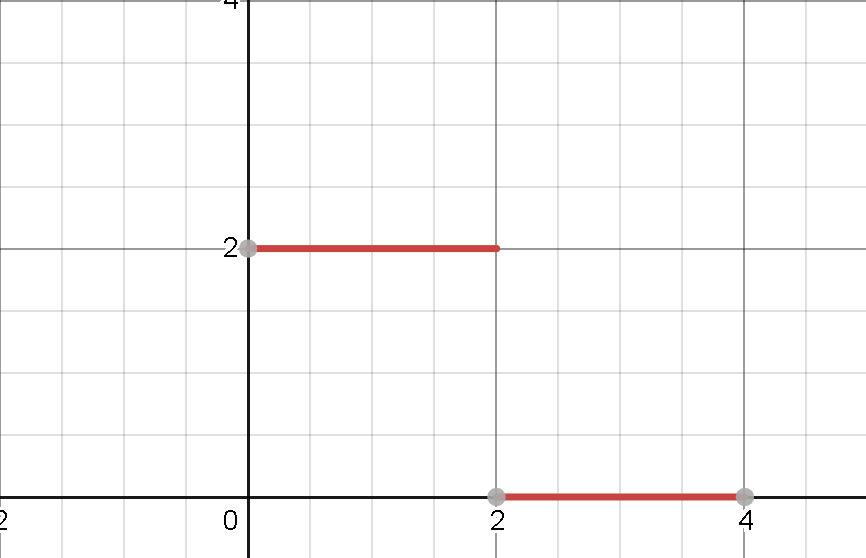
\includegraphics[width=0.6\textwidth]{baseGraph.png}
\end{figure}

We can see that $f(x)$ is periodic with a period of 4.

Let's use the partial sum of the Fourier series to construct a function that approaches $f(x)$ over the domain from 0 to T (and for its repeating cycles)

Continuing with Desmos, we write the synthesis equation of the Fourier series and plug in the integrals of the coefficients in their places. After we have shortened the expression, we are now looking at the following expression, which we can then fill in in the second field of Desmos:

\begin{equation*}
	\frac{1}{T}\int_{0}^{2}2\;dx + \sum\limits_{n=1}^k \frac{2}{T}\int_{0}^{2}2cos\frac{2\pi kx}{T}\;dx\;cos\frac{2\pi kx}{T} + \sum\limits_{n=1}^k \frac{2}{T}\int_{0}^{2}2sin\frac{2\pi kx}{T}\;dx\;sin\frac{2\pi kx}{T}
\end{equation*}
$k$ is the number of terms (excluding the constant term) we will take when calculating the partial sum.

If we choose the number of terms to be 4 (so $n$, or as denoted in the picture, $k$, equals $3$):

\begin{figure}[H]
	\centering
	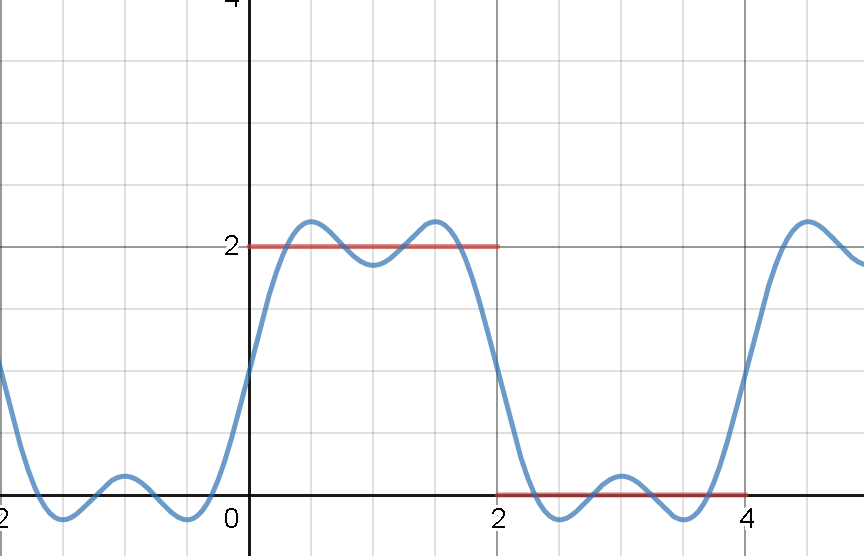
\includegraphics[width=0.6\textwidth]{k=3.png}
\end{figure}

We can see that the new function somewhat resembles $f(x)$.

As we add more terms, it comes even closer and closer to becoming $f(x)$.

With $k = 7$:
\begin{figure}[H]
	\centering
	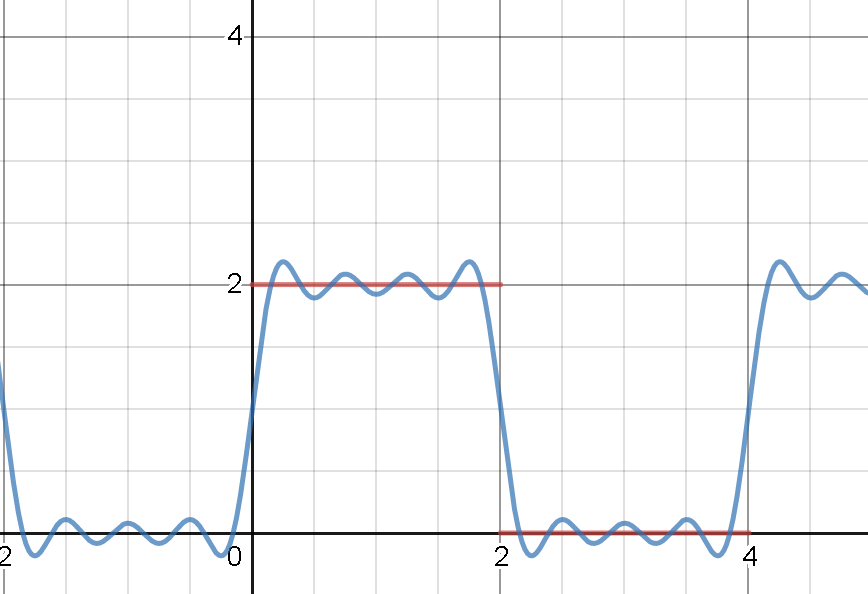
\includegraphics[width=0.6\textwidth]{k=7.png}
\end{figure}

With $k = 11$:
\begin{figure}[H]
	\centering
	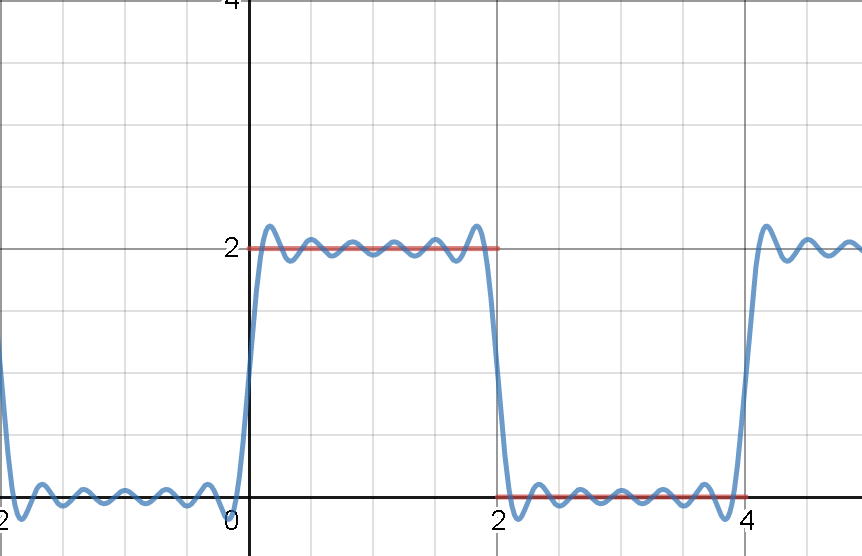
\includegraphics[width=0.6\textwidth]{k=11.png}
\end{figure}
\newpage
With $k = 21$:
\begin{figure}[H]
	\centering
	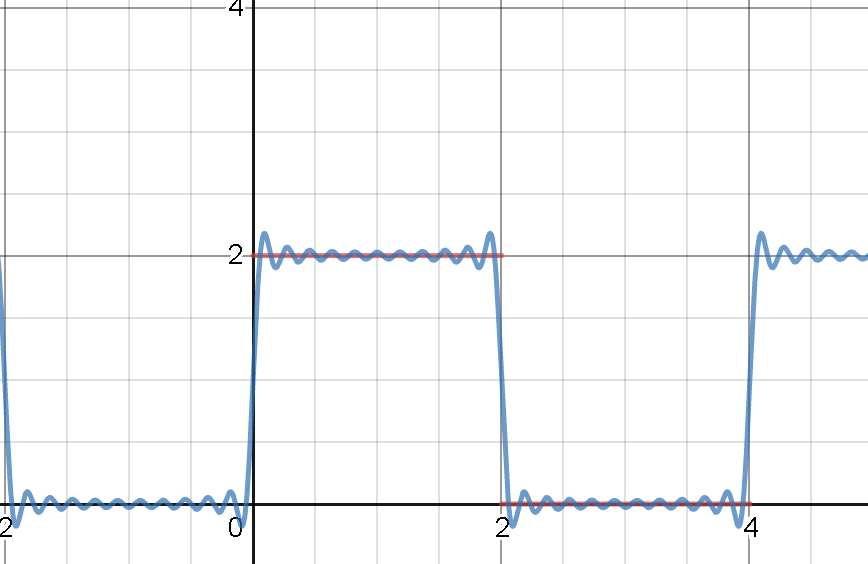
\includegraphics[width=0.6\textwidth]{k=21.png}
\end{figure}

With $k = 35$:
\begin{figure}[H]
	\centering
	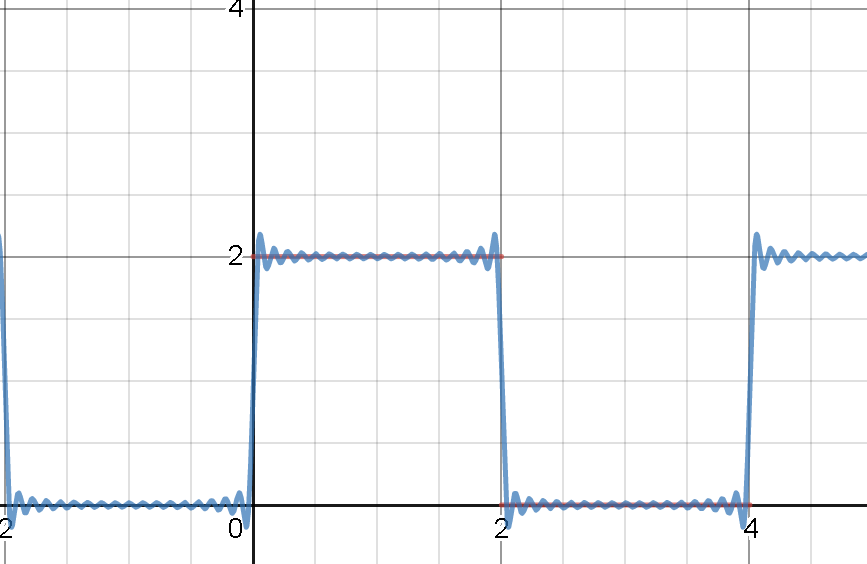
\includegraphics[width=0.6\textwidth]{k=35.png}
\end{figure}

So, we can say with confidence, that when $n$ approaches infinity, the sum of this Fourier series will converge to $f(x)$.

One thing we can note here is: as more terms are added, the frequency of those terms approach infinity. This will ensure that the final summation of the series will cover just about every corner of the frequency spectrum.

But, not everyone can take full advantage of having full resolution of the picture (or in this particular application, full spectrum of the audio wave). There is a limit to human's perception, and those outside of that perceiving range are often subconsciously discarded by our brain during the receiving and processing phase. By utilizing that fact, we can remove the unnecessary, insignificant bits of the original data while still retaining the important parts that are easily recognizable by the human mind, thus reducing the size of that data while still keeping the relevant contents. And that is what data compression essentially is.

So, for instance, the hearing range of human's ears are from 16Hz to 20kHz. By eliminating terms with frequency beyond that point, we have successfully cut down on the size of the data while making practically no changes to quality because we more than often are unable to perceive them anyway. Even better yet, human's sensitive range of hearing, where we can normally discern the sounds being played without too much attention to details, is only from 2kHz to 5kHz. That makes it so that unless people try to deliberately be on the lookout for artefacts, we can reduce the number of terms even further to achieve greater result in reducing the size of the original data. 

\newpage
\subsection{$\mathit{e}$ (Mathematical Constant)}
The number $\mathit{e}$ is a mathematical constant approximately equal to $2.71828$ and is the base of the natural logarithm. It is the limit of $(1+\frac{1}{n})^n$ as $n$ approaches infinity. It can also be calculated as the sum of the infinite series
\begin{equation*}
	\mathit{e} = \sum_{n=0}^{\infty}\frac{1}{n!}
\end{equation*}

The number $\mathit{e}$ has extreme importance in mathematics, alongside $0$, $1$, $\pi$ and $\mathit{i}$. $\mathit{e}$ is a big deal because it is the natural language of growth. It is the only function where $y(x)=\mathit{e}^x$, $y\prime(x)=\mathit{e}^x$ and $\int \mathit{e}^x\;dx = \mathit{e}^x$. Thus, anything related to growth written in terms of $\mathit{e}$ is much simpler.

\pdfbookmark[1]{$\mathit{e}$ (Compound Interest)}{euler}
The discovery of $\mathit{e}$ is a very good example. An account starts with $\$1.00$ and pays 100 percent interest per year. If the interest is credited once, at the end of the year, the value of the account at year-end will be $\$2.00$. What happens if the interest is computed and credited more frequently during the year?\\\\
If the interest is credited twice a year, the interest rate for each 6 months will be $50\%$, so at the end of the year, the total value in the account is
\begin{equation*}
	\$1.00 \cdot 1.5^2 = \$2.25
\end{equation*}
Compounding quarterly yields
\begin{equation*}
	\$1.00 \cdot (1 + 1/12)^{12} = \$2.613...
\end{equation*}
If there are $n$ compounding intervals, the interest for each interval will be $1/n$ and the value at the end of the year will be $\$1.00\cdot(1+1/n)^n$. Bernoulli noticed that this sequence approaches a limit with larger $n$, which is now called the natural base $\mathit{e}$.
\begin{figure}[H]
	\centering
	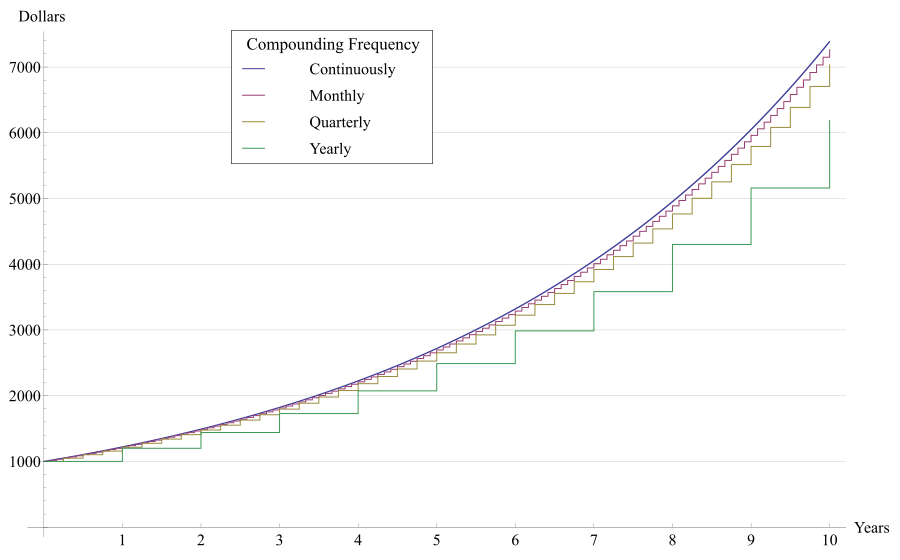
\includegraphics[width=0.8\textwidth]{euler1.png}
\end{figure}

\newpage
\bibliography{Assignment.bib}
\bibliographystyle{ieeetr}
\end{document}